\begin{ledgroupsized}[r]{120mm}
\footnotesize
\pstart
\noindent\textbf{Überlieferung:}
\pend
\end{ledgroupsized}
\begin{ledgroupsized}[r]{114mm}
\footnotesize
\pstart
\parindent -6mm
\makebox[6mm][l]{\textit{L}}%
Konzept:
LH~XXXVII~3~Bl.~75\textendash76. 
Ein Bogen~2\textsuperscript{o}; 
\href{\Scan{LH_37_03_075wz}}%
{Wasserzeichen} in Bl.~75.
Vier unregelmäßig beschriebene Seiten.
Die obere Hälfte von Bl.~76~v\textsuperscript{o} überliefert Rechnungen und eine Zeichnung (in Bleistift, wohl von Leibnizens Hand) ohne Bezug zum Text. Diese sind tlw. überschrieben und müssen vor dem Text enstanden sein.
\pend
\end{ledgroupsized}
\selectlanguage{latin}
\vspace{8mm}
\pstart
\centering
\edlabel{37_03_075-076_1a}%
\edtext{}{%
\xxref{37_03_075-076_1a}{37_03_075-076_1b}%
\lemma{\href{\Scan{LH_37_03_075r}}%
{\lbrack75~r\textsuperscript{o}\rbrack}}%
\Bfootnote{%
\bars{\textit{(1)}~De %
\textit{(a)}~rotis %
\textit{(b)}~figuris dent  %
\textit{(2)}~De vectibus \lbrack...\rbrack\ cogitationes
\bars{scheda 1\textsuperscript{ma}. \textit{erg.}}
25 Octobr. 1679.~\textit{erg.}}
\lbrack/\rbrack\
\textit{(1)}~Sit Triangulum isosceles %
\textit{(a)}~ \textit{ADC} %
\textit{(b)}~\textit{BCD} sumtaque in recta \textit{BD} producta alio puncto \textit{A} junctaeque %
\textit{(2)}~In Triangulo~\textit{L}}}%
\href{\Scan{LH_37_03_075r}}%
{\lbrack75~r\textsuperscript{o}\rbrack}
\hfill
De vectibus\indexS{vectes conjugati} conjugatis et figuris\indexS{figurae dentium} dentium in \indexS{rota}rotis,
\hfill
\phantom{\lbrack75~r\textsuperscript{o}\rbrack}
\linebreak
resumtae
\edtext{priores cogitationes}{%
\applabel{FnC:37_03_075-076_resumtae}%
\lemma{priores cogitationes}\Cfootnote{Gemeint sind vier, mit N.\;\ref{57034} inhaltlich verwandte und in der benachbarten Signatur LH XXXVII 3, Bl.~77\textendash80 überlieferte Konzepte \cite{02160}"De vectibus conjugatis" aus der zweiten Hälfte von 1674 (\textit{LSB} VIII,~2 N.\;45).}}
scheda 1\textsuperscript{ma}. 25 Octobr. 1679.
\pend
\nobreak
\vspace{0.5\baselineskip}
\begin{edfigure}%
\includegraphics[scale=1]{%
gesamttex/edit_VIII-4/images/LH_37_03_075-076_d1_075r.pdf}
\edcaption[-.1em]{%
\edtext{\lbrack\textit{Fig.~1, tlw. Blindzeichnung}\rbrack}{%
\lemma{}%
\Afootnote[nonum]{\textit{Neben \bracks{\textit{Fig.~1}}}: Brevior vectis potentior}}}
\end{edfigure}
\pstart
\noindent
In Triangulo\indexS{triangulum}\edlabel{37_03_075-076_1b}
\textit{BCD} sint latera \textit{BC}, \textit{BD} aequalia, producatur \textit{BD} usque in \textit{A}, junctaeque \textit{AC}, sumatur in \textit{AB} aequalis \textit{AE} ita ut juncta \textit{CE} fiat aliud triangulum\indexS{triangulum isosceles} isosceles \textit{ACE}, quaeritur ratio inter \textit{CD} et \textit{CE}.
\pend
\pstart
\textls{%
$\left.\begin{array}{c}AC\\AE\end{array}\!\!\right\}$
sit \textit{a}, \textit{CE} sit \textit{e}\bracks{;}}
\textit{CG} erit $\displaystyle\frac{e}{2}$, \textit{AG} erit $\sqrt{a^2-\displaystyle\frac{e^2}{4}}$ 
vel $\displaystyle\frac{\sqrt{4a^2-e^2}}{2}$ 
et area Trianguli \textit{ACE} erit $\displaystyle\frac{e\sqrt{4a^2-e^2}}{4}$, eadem
\edtext{est \textit{AE}}{%
\lemma{est}%
\Bfootnote{%
\textit{(1)}~\textit{AF} in %
\textit{(2)}~\textit{AE}~\textit{L}}}
in \textit{CF}, seu \textit{a} in \textit{CF}, ergo erit 
\textls{\textit{CF} aequ. $\displaystyle\frac{e\sqrt{4a^2-e^2}}{4a}$.}
\pend
\pstart
Eodem
\edtext{modo ponendo}{%
\lemma{modo}%
\Bfootnote{%
\textit{(1)}~quaerendo %
\textit{(2)}~ponendo~\textit{L}}}
\rule[-3.1ex]{0pt}{4ex}%
\textls{$\left.\begin{array}{c}BC\\BD\end{array}\!\!\right\}$ 
esse \textit{b}} 
et 
\textls{\textit{CD} esse \textit{d}}
quaerendoque
\edtext{similiter altitudinem}{%
\lemma{similiter}%
\Bfootnote{%
\textit{(1)}~perpendicularem \textit{CF}, e %
\textit{(2)}~altitudinem~\textit{L}}}
\textit{CF} in Triangulo \textit{BCD}, uti quaesiveramus in Triangulo \textit{ACE}, fiet \textls{\textit{CF} aequ.}
\rule[-1.8ex]{0pt}{5.4ex}%
$\displaystyle\frac{d\sqrt{4b^2-d^2}}{4b}$.
\pend
\pstart
Quos duos valores aequando, fiet: $be\sqrt{4a^2-e^2}\sqcap ad\,\sqrt{4b^2-d^2}$ sive $4a^2b^2e^2-b^2e^4\sqcap 4a^2b^2d^2-a^2d^4$\bracks{,} qua aequatione satis exprimitur relatio inter \textit{a}, \textit{b}, \textit{e}, \textit{d}.
\pend
\pstart
Ponamus jam \textit{d} et \textit{e} esse infinite parvas, tunc utique evanescent termini $b^2e^4$, et $a^2d^4$, et restabit $4a^2b^2e^2\sqcap 4a^2b^2d^2$ sive fiet $d\sqcap e$.
\edtext{}{%
\lemma{}\Afootnote{\textit{Am Rand}:\quad 
\raisebox{-1ex}{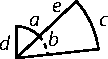
\includegraphics[scale=1]{gesamttex/edit_VIII-4/images/LH_37_03_075-076_d2_075r.pdf}}\enskip \lbrack\textit{Fig.~2}\rbrack\textsuperscript{\bracks{a}}\\
$\displaystyle\frac{c}{b}\sqcap\displaystyle\frac{e}{d}$. $b\sqcap\displaystyle\frac{dc}{e}$.\raisebox{.5ex}{\textsuperscript{\bracks{b}}}
$\displaystyle\frac{a}{b}\sqcap\doublefrac{a}{\dfrac{dc}{e}}$. Ergo $\displaystyle\frac{a}{b}\sqcap\displaystyle\frac{ae}{cd}$.\raisebox{.5ex}{\textsuperscript{\bracks{c}}} 
Ergo anguli \textit{a}, \textit{b} inter se in ratione composita ex directa\textsuperscript{\lbrack d\rbrack} arcuum \textit{a}, \textit{c} et reciproca radiorum \textit{e}, \textit{d}.
\\[1.5ex] 
{\footnotesize 
\textsuperscript{\lbrack a\rbrack}\bracks{\textit{Fig.~2}}: Ein nicht gestrichener Entwurf zum Diagramm wird nicht wiedergegeben.
\textsuperscript{\lbrack b\rbrack}$b\sqcap\displaystyle\frac{dc}{e}$. %
\textit{(1)}~$\displaystyle\frac{a}{c}\sqcap\doublefrac{a}{\dfrac{eb}{c}}$ %
\textit{(2)}~$\displaystyle\frac{a}{b}\sqcap\doublefrac{a}{\dfrac{dc}{e}}$~\textit{L}\quad
\textsuperscript{\lbrack c\rbrack}$\displaystyle\frac{a}{b}\sqcap\displaystyle\frac{ae}{cd}$. %
\textit{(1)}~anguli %
\textit{(a)}~arcus vel anguli %
\textit{(b)}~\textit{a}, \textit{b} inter se %
\textit{(2)}~Ergo~\textit{L}\quad
\textsuperscript{\lbrack d\rbrack}directa %
\textit{(1)}~radiorum %
\textit{(2)}~arcuum~\textit{L}}}}
\pend
\pstart
Hinc sequitur duos vectes conjugatos in directum
\edtext{sitos aequali potentia recta descendente se prementes, agere potentia longitudini brachiorum reciproca.}{%
\lemma{sitos}%
\Bfootnote{%
\textit{(1)}~aequali potentia se prementes, 
\textit{(a)}~in aequilibrio esse %
\textit{(b)}~agere
\textit{(2)}~se potentia
\textit{(3)}~aequali \bracks{...} agere potentia
\textit{(a)}~longitudines
\textit{(b)}~longitudinis brachiorum reciproca.~\textit{L}}}
Sive si sint duo vectes \textit{AE}, \textit{BD}, mobiles circa centra \textit{A}, \textit{B} quorum ille deprimitur a pondere \textit{L}, hic a pondere \textit{M} attollitur et si pondera\indexS{pondera aequalia} sint
\edtext{aequalia et ex aequalibus trochleis\indexS{trochlea} suspensa, et in linea recta descendant}{%
\lemma{et}%
\Bfootnote{%
\textit{(1)}~aequalia %
\textit{(2)}~aequalis %
\textit{(3)}~aequali a centro \textit{A} distantia suspensa, %
\textit{(4)}~ex aequalibus trochleis %
\textit{(a)}~suspensas %
\textit{(b)}~suspensa, \bars{et ita \textit{streicht Hrsg.}} et in linea recta descendant~\textit{L}}}
ita, ut discrimen sit tantum in vectium
\edtext{longitudine \textit{AE}, \textit{BD} inaequali. Vincet pondus, quod magis descendit\lbrack,\rbrack\ id est quod majorem arcum trochleae circumagit, id est quod majorem evolvit fili partem. Sunt autem anguli \textit{A}, \textit{B} inter se in ratione composita ex directa arcuum, et reciproca radiorum. Sed initio positis rectis}{%
\lemma{longitudine \textit{AE}, \textit{BD}}%
\Bfootnote{%
\textit{(1)}~inaequali, ajo %
\textit{(a)}~hoc %
\textit{(b)}~hac non obstante aequilibrium fore; nam %
\textit{(aa)}~ut %
\textit{(bb)}~ut brachium longius \bars{\textit{BD} \textit{erg.}} vincat, debet extremitas ejus \textit{D} majorem %
\textit{(aaa)}~circulum describere \textit{DE} %
\textit{(bbb)}~arcum \textit{DE} describere, quam est arcus \textit{EC}, quem describit extremitas \textit{E} vectis brevioris \textit{AE}, ita enim pondus \textit{M} magis descendit quam pondus \textit{L}. Sed initio positis %
\textit{(2)}~inaequali. Vincet pondus, quod magis descendit id est quod %
\textit{(a)}~majorem 
\textit{(aa)}~\bars{angulum \textit{streicht Hrsg.}}
\textit{(bb)}~arcum
\textit{(cc)}~arcum trochleae
\textit{(aaa)}~evolvit, id enim majorem circum
\textit{(bbb)}~circum
\textit{(ccc)}~circumagit, \bracks{...} positis rectis~\textit{L}}}
\textit{DC}, \textit{EC} infinite parvis calculus ostendit eas esse aequales (quod alioqui ut in sequentibus ostendam etiam infinite parvis fieri non solet).
\edtext{Itaque et arcus quibus rectae \textit{DE}, \textit{CE} subtenduntur sunt aequales, adeoque sublata ratione arcuum directa manet ratio radiorum seu vectium reciproca, quare}{%
\lemma{Itaque}%
\Bfootnote{%
\textit{(1)}~aequalis est ab initio nisus sive descendendi potentia utrinque, quare %
\textit{(2)}~et arcus quibus \bars{rectae \textit{erg.}} \textit{DE}, \bracks{...} ratio %
\textit{(a)}~radiorum %
\textit{(b)}~radiorum seu vectium reciproca, \bars{quare \textit{streicht Hrsg.}} quare~\textit{L}}}
\textls{duo vectes conjugati in directum positi utcunque longitudine inaequales, si modo aequali utrinque}
\edtext{\textls{ponderis recta descendentis gravitatione sibi contranitantur} potentiam habebunt in reciproca longitudinum ratione.}{%
\lemma{\textls{utrinque}}%
\Bfootnote{%
\textit{(1)}~vi agantur %
\textit{(2)}~in contra %
\textit{(3)}~si %
\textit{(4)}~vi %
\textit{(5)}~\textls{ponderis} \bars{\textls{recta descendentis} \textit{erg.}} \textls{gravitatione sibi contranitantur} %
\textit{(a)}~\textls{in aequilibrio manebunt} %
\textit{(b)}~potentiam habebunt in reciproca longitudinum ratione.~\textit{L}}}
Ipsi autem vectes per se hic pondere semper carere ponuntur, vel 
\edtext{ab eodem pondere animus}{%
\lemma{ab}%
\Bfootnote{%
\textit{(1)}~eo
\textit{(2)}~eodem pondere
\textit{(a)}~animo
\textit{(b)}~animus~\textit{L}}}
abstrahitur.
\pend
\pstart
\href{\Scan{LH_37_03_075v}}%
{\lbrack75~v\textsuperscript{o}\rbrack}\ 
\edtext{Caeteris ut ante positis}{%
\lemma{}%
\Bfootnote{Caeteris ut ante positis \textit{erg.~L}}}
sint jam duo vectes conjugati \textit{AE}, \textit{BD} non in directum siti, sed angulum facientes in \textit{D} seque ducentes in eodem plano in quo sunt siti. \textit{BD} describet arcum \textit{DC}, et \textit{AE}
\edtext{arcum \textit{EC}. Quaeritur horum}{%
\lemma{arcum \textit{EC}.}%
\Bfootnote{%
\textit{(1)}~Manifestum est vires exercitas esse ut ponderum descensus, quia autem pondera \bars{\textit{L}, \textit{M} \textit{erg., streicht Hrsg.}} ex trochleis \bars{aequalibus \textit{erg.}} %
\textit{(a)}~\textit{A}, \textit{B} circa %
\textit{(b)}~circa \textit{A}, \textit{B} 
\bars{\textit{(1)}~filis
\textit{(2)}~filo \textit{erg.}} 
suspensa intelliguntur; hinc %
\textit{(aa)}~tantam portione %
\textit{(bb)}~tantum descendit pondus \textit{L} vel \textit{M}, quantum est filum quod evolvitur trochlea circumacta, %
\textit{(aaa)}~trochlea autem, e %
\textit{(bbb)}~id est quantus est trochleae arcus, is autem tantus est quantus est angulus %
\textit{(2)}~Quaeritur horum~\textit{L}}}
arcum\indexS{ratio arcuum} ratio. %
\pend
\pstart
Cum sint infinite parvi eadem erit quae subtensarum; subtensa autem arcus infinite parvi haberi potest pro portione
\edtext{tangentis. Ergo}{%
\lemma{tangentis}%
\Bfootnote{%
\textit{(1)}~, productae %
\textit{(2)}~. Ergo~\textit{L}}}
\textit{CD}, \textit{CE}
\edtext{cum circulos tangant in \textit{C} angulos facient}{%
\lemma{cum}%
\Bfootnote{%
\textit{(1)}~arcus circuli %
\textit{(2)}~circulos tangant
\textit{(a)}~in %
\textit{(aa)}~\textit{C} et %
\textit{(bb)}~\textit{D} et \textit{E} 
\textit{(aaa)}~productae
\textit{(bbb)}~si producantur in \textit{Q}, \textit{P} erunt anguli ipsarum %
\textit{(cc)}~\textit{C} sive \bars{in \textit{gestr.}} \textit{C}, \textit{D}, \textit{E} %
\textit{(dd)}~si producantur %
\textit{(aaa)}~angulos %
\textit{(bbb)}~in \textit{Q}, \textit{P} %
\textit{(ccc)}~\bars{in \textit{C}, \textit{D}, \textit{E} \textit{erg.}} angulos fa %
\textit{(b)}~in \textit{C} angulos facient~\textit{L}}}
rectos ad radios
\edtext{suos \textit{BC}, \textit{AC} sive si producantur}{%
\lemma{suos}%
\Bfootnote{%
\textit{(1)}~\textit{AC} vel \textit{AE} aut \textit{BC} vel \textit{BD}
\textit{(2)}~\textit{BC}, \textit{AC}
\textit{(a)}~vel \textit{A}, \textit{E} et %
\textit{(b)}~\textit{BC} %
\textit{(c)}~\textit{AC} %
\textit{(aa)}~vel \textit{BD} %
\textit{(bb)}~sive si producantur~\textit{L}}}
in \textit{P}, \textit{Q} erunt
\edtext{anguli \textit{BCQ} sive \textit{BDQ}}{%
\lemma{anguli}%
\Bfootnote{%
\textit{(1)}~\textit{ACP} sive \textit{AEP} %
\textit{(2)}~\textit{BCQ} sive \textit{BDQ}~\textit{L}}}
(nam puncta \textit{C}, \textit{D} eatenus pro coincidentibus
\edtext{habentur) recti}{%
\lemma{habentur)}%
\Bfootnote{%
\textit{(1)}~recti, vel \textit{ADR} %
\textit{(2)}~recti~\textit{L}}}
itemque anguli \textit{ACP} sive \textit{AEP}, sive \textit{ADR}. Ducatur ipsi \textit{AD} parallela, \textit{BRQ}\bracks{,} erit triangulum \textit{QDR} simile Triangulo \textit{DCE}. Erit ergo \textit{DC}
\edtext{ad \textit{EC} subtensa}{%
\lemma{ad \textit{EC}}%
\Bfootnote{%
\textit{(1)}~sive arcus ad arcum %
\textit{(2)}~subtensa~\textit{L}}}
ad subtensam, sive quod hic idem est, arcus ad arcum, ut \textit{QD} ad \textit{PR}. Angulus ergo \textit{CAE}, est 
\edtext{ad angulum \textit{CBD}}{%
\lemma{ad angulum}%
\Bfootnote{%
\textit{(1)}~\textit{BD}
\textit{(2)}~\textit{CBD}~\textit{L}}}
in ratione
\edtext{directa}{%
\lemma{}%
\Bfootnote{directa \textit{erg.~L}}}
arcuum \textit{CE}, \textit{CD}, sive rectarum \textit{DR}, \textit{DQ}, et reciproca\indexS{ratio reciproca radiorum} radiorum, seu in ratione \textit{BD} ad \textit{AD}. 
Regulam ergo hanc praescribemus: sint duo vectes\indexS{vectes conjugati} conjugati, qui ponderibus\indexS{pondus} ex aequalibus trochleis\indexS{trochlea} pendentibus circumaguntur, sibique obnituntur
\edtext{in \textit{D}, manentes}{%
\lemma{in \textit{D},}%
\Bfootnote{%
\textit{(1)}~in eodem plano %
\textit{(2)}~manentes~\textit{L}}}
\edtext{plano. Uni vectium \textit{AE}, ducatur}{%
\lemma{plano}%
\Bfootnote{%
\textit{(1)}~Ipsi vecti ducendo %
\textit{(2)}~Uni vectium %
\textit{(a)}~ducatur %
\textit{(b)}~\textit{AE}, %
\textit{(aa)}~ab %
\textit{(bb)}~ducatur~\textit{L}}}
in eodem invicem per alterius centrum \textit{B}
\edtext{parallela \textit{BRQ}}{%
\lemma{parallela}%
\Bfootnote{%
\textit{(1)}~\textit{BR} %
\textit{(2)}~\textit{BRQ}~\textit{L}}}
cui ex
\edtext{puncto \textit{D} vectibus ad angulos rectos eductae}{%
\lemma{puncto \textit{D}}%
\Bfootnote{%
\textit{(1)}~ad angulos rectos 
\textit{(a)}~tam ipsi \textit{A} 
\textit{(b)}~utrique vectium %
\textit{(2)}~vectibus \bars{ad angulos rectos \textit{erg.}}
eductae~\textit{L}}}
\textit{DR}, \textit{DQ}, occurrant in punctis
\edtext{\textit{R}, \textit{Q}, erit}{%
\lemma{\textit{R}, \textit{Q},}%
\Bfootnote{%
\textit{(1)}~erunt potentiae vectium %
\textit{(2)}~erit~\textit{L}}}
potentia vectis \textit{AD} contra potentiam\indexS{potentia} vectis \textit{BD} in composita ratione
\edtext{ex rationibus}{%
\lemma{ex}%
\Bfootnote{%
\textit{(1)}~ratione %
\textit{(2)}~rationibus~\textit{L}}}
\textit{DR} ad \textit{DQ} et \textit{DB} ad \textit{DA}. 
Seu ratio exercitii potentiarum \textit{L}, et \textit{M} erit ut \textit{BD}, \textit{DR} ad \textit{AD}, \textit{DQ} seu \rule[-4mm]{0pt}{10mm}$\displaystyle\frac{\text{pot.}\; L}{\text{pot.}\; M}\sqcap\displaystyle\frac{BD, DR}{AD, DQ}$.
\pend
\pstart
Si Angulus \textit{ADB} nullus seu infinite obtusus, 
\edtext{seu si \textit{ADB} recta}{%
\lemma{seu si}%
\Bfootnote{%
\textit{(1)}~\textit{AB}, \textit{DB} %
\textit{(2)}~\textit{ABD} recta %
\textit{(3)}~\textit{ADB} recta~\textit{L}}}
una, coincident \textit{DQ}, \textit{DR} quippe ad hanc rectam perpendiculares,
\edtext{coincidet et recta \textit{AB} ipsi \textit{ADB},}{%
\lemma{}%
\Bfootnote{coincidet et recta \textit{AB} ipsi \textit{ADB} \textit{erg.~L}}}
adeoque sublata ratione \textit{DR}, \textit{DQ} remanebit sola \textit{BD}, \textit{AD}, seu ratio pot. \textit{L} ad pot. \textit{M} erit \textit{BD} ad \textit{AD}, nempe reciproca
\edtext{radiorum. Quod}{%
\lemma{radiorum}%
\Bfootnote{%
\textit{(1)}~, 
\textit{(a)}~ut
\textit{(b)}~ut supra %
\textit{(2)}~. Quod~\textit{L}}}
jam supra alia methodo ostenderamus.
\pend
\pstart
Si
\edtext{jam vectium}{%
\lemma{jam}%
\Bfootnote{%
\textit{(1)}~dens vel vectis %
\textit{(2)}~vectium~\textit{L}}}
conjugatorum alteruter,
\edtext{ut \textit{ACS}}{%
\lemma{}%
\Bfootnote{ut  \bars{dens \textit{gestr.}} \textit{ACS}~\textit{L}}}
non sit
\edtext{linea}{%
\lemma{}%
\Bfootnote{linea \textit{erg.~L}}}
recta, sed vel curva, vel ex recta una in plures fracta, quod et in curva intelligi potest,
\edtext{quae componi intelligitur ex recta in infinitas partes}{%
\lemma{quae}%
\Bfootnote{%
\textit{(1)}~semper est infi %
\textit{(2)}~rect %
\textit{(3)}~componi intelligitur ex recta in infinitas %
\textit{(a)}~curvas fracta %
\textit{(b)}~partes~\textit{L}}}
fracta, res eodem redit. Nempe ponatur vectis curvus vel flexus \textit{ACS} ab altero \textit{BC} duci in \textit{ACT}. erunt potentiae, ut anguli \textit{TAS}, \textit{TBC}, seu in ratione \textit{TS}, \textit{TC} directa, et radiorum reciproca, ducatur ipsi \textit{CS} fragmento seu portioni vectis fracti ducendae, seu si vectis curva linea constat. Ducatur Tangenti ejus
\edtext{curvae (quae curvam contingat}{%
\lemma{curvae~(}%
\Bfootnote{%
\textit{(1)}~quae est %
\textit{(2)}~quae curvam contingat~\textit{L}}}
in puncto ubi sibi vectis ille ab alio impellitur) parallela per punctum \textit{B}, nempe \textit{BVX}, cui productae \textit{TSV}, \textit{TCX} occurrant\bracks{,} id est perpendiculares ad \textit{AT}, \textit{BT} seu \textit{AC}, \textit{BC}. Coincidere enim intelliguntur puncta \textit{C}, \textit{T}, \textit{S}. Erit angulus ad angulum, 
\edlabel{37_03_075-076_3a}%
\edtext{}{%
\xxref{37_03_075-076_3a}{37_03_075-076_3b}%
\lemma{}%
\Bfootnote{%
\textit{(1)}~\href{\Scan{LH_37_03_076r}}%
{\lbrack76~r\textsuperscript{o}\rbrack} potentia \textit{L} ad potentiam \textit{M}, ut
\textit{(a)}~\textit{BD}
\textit{(b)}~\textit{BC}
\textit{(c)}~ \textit{BT}, \textit{TX} ad \textit{AT}, \textit{TV}.
\textit{(2)}~potentia \bracks{...} \textit{TV}. \href{\Scan{LH_37_03_076r}}%
{\lbrack76~r\textsuperscript{o}\rbrack} Quaeritur~\textit{L}}}%
seu potentia \textit{L} ad potentiam \textit{M}, ut \textit{BT}, \textit{TX} ad \textit{AT}, \textit{TV}.
\pend
\pstart\noindent
\href{\Scan{LH_37_03_076r}}%
{\lbrack76~r\textsuperscript{o}\rbrack}\ 
\pend
\begin{edfigure}[0em][1em]
\includegraphics[scale=1]{%
gesamttex/edit_VIII-4/images/LH_37_03_075-076_d3_076r.pdf}
\edcaption[-.25em]{\edtext{\lbrack\textit{Fig.~3}\rbrack}{%
\lemma{}\Afootnote[nonum]{\textit{Unter \bracks{Fig.~3}, gestrichen}: potentia \textit{L} ad potentiam \textit{M}, ut\textsuperscript{\lbrack a\rbrack} \textit{BT}, \textit{TX} ad \textit{AT}, \textit{TV}.
\\[1.5ex] 
{\footnotesize \textsuperscript{\lbrack a\rbrack} ut %
\textit{(1)}~\textit{BD} %
\textit{(2)}~\textit{BC} %
\textit{(3)}~\textit{BT}~\textit{L}}}}}
\end{edfigure}
\pstart
\edtext{}{%
\lemma{}\Afootnote{\textit{Neben} \lbrack\textit{Fig.~3}\rbrack: Nota: Brevior vectis potentior, ideo figura nonnihil immutanda, vel in contraria trochlearum parte locanda pondera, ut non attollat\textsuperscript{\lbrack a\rbrack} vectis \textit{BD} vectem \textit{AE} sed deprimat\textsuperscript{\lbrack b\rbrack} vectis \textit{AE} vectem \textit{AD}.\\[1.5ex] 
{\footnotesize 
\textsuperscript{\lbrack a\rbrack}attollat %
\textit{(1)}~\textit{BC} \textit{AE}
\textit{(2)}~vectis \textit{BD} vectem \textit{AD}~\textit{L}\quad
\textsuperscript{\lbrack b\rbrack}deprimat %
\textit{(1)}~\textit{AE} %
\textit{(2)}~\textit{AE} %
\textit{(3)}~vectis \textit{AE}~\textit{L}}}}
Quaeritur\edlabel{37_03_075-076_3b} 
jam qualisnam debeat esse curva, seu flexio\indexS{flexio vectis} vectis sive \indexS{flexio dentis}dentis \textit{ACS} talis,
\edtext{ut eadem}{%
\lemma{ut}%
\Bfootnote{%
\textit{(1)}~ea
\textit{(2)}~aequalis semper %
\textit{(3)}~eadem~\textit{L}}}
semper maneat ratio\indexS{ratio potentiarum} potentiarum, sive quod idem est angulorum\indexS{ratio angulorum} vel revolutionum\indexS{ratio revolutionum}, id vero non difficulter 
\edlabel{37_03_075-076_2a}%
\edtext{}{%
\xxref{37_03_075-076_2a}{37_03_075-076_2b}%
\lemma{fiet}%
\Bfootnote{%
\textit{(1)}~sive per puncta, sive etiam continuo tractu. %
\textit{(a)}~Hoc modo: %
\textit{(b)}~Et primum per puncta hoc modo: %
\textit{(2)}~Moveatur~\textit{L}}}%
fiet.
\pend
\pstart
Moveatur\edlabel{37_03_075-076_2b}
planum $\Omega$ circa centrum \textit{A},
\edtext{et recta}{%
\lemma{et}%
\Bfootnote{%
\textit{(1)}~vectis %
\textit{(2)}~recta~\textit{L}}}
\textit{BD} circa centrum \textit{B} et quidem
\edtext{vectis}{%
\lemma{}%
\Bfootnote{vectis \textit{erg.~L}}}
\textit{B} triplo celerius quam planum, in puncto vectis \textit{D}. Sit stylus describens curvam in
\edtext{plano $A\gimel\beth\aleph D$ $\aleph\beth\gimel D$.}{%
\lemma{plano}%
\Bfootnote{%
\textit{(1)}~\textit{DCA} %
\textit{(2)}~\bars{$\aleph\beth\gimel D$ \textit{streicht Hrsg.}}
\textit{(3)}~$A\gimel\beth\aleph D$~\textit{L}}}
Ea curva erit quaesita nempe dens sive vectis 
\edtext{erit $A\gimel\beth\aleph D$.}{%
\lemma{erit}%
\Bfootnote{%
\textit{(1)}~\textit{ADCS} %
\textit{(2)}~\textit{$A\aleph\beth\gimel D$} %
\textit{(3)}~$A\gimel\beth\aleph D$.~\textit{L}}}
\pend
\begin{edfigure}%
\includegraphics[scale=1]{%
gesamttex/edit_VIII-4/images/LH_37_03_075-076_d4_076r.pdf}%
\hspace*{2.5em}
\edcaption{\bracks{\textit{Fig.~4}}}
\end{edfigure}
\pstart
Si rotae duae
\edtext{se ducentes in quibus figura dentium quaeritur}{%
\lemma{}%
\Bfootnote{se ducentes %
\textit{(1)}~\bars{de \textit{streicht Hrsg.}}
\textit{(2)}~quarum dentes %
\textit{(3)}~figur %
\textit{(4)}~in quibus figura dentium quaeritur \textit{erg.~L}}}
non sint in eodem plano, ut rotae \textit{S}, \textit{T}, figura dentium eodem modo quaeri
\edtext{potest. Hoc}{%
\lemma{pot\-est}%
\Bfootnote{%
\textit{(1)}~, nam %
\textit{(2)}~. Hoc~\textit{L}}}
ita fiet:
\pend
\begin{edfigure}%
\includegraphics[scale=1]{%
gesamttex/edit_VIII-4/images/LH_37_03_075-076_d5_076r.pdf}
\edcaption[.1em]{\lbrack\textit{Fig.~5}\rbrack}
\end{edfigure}
\pstart
Dum
\edtext{rota \textit{T} vel ejus dens \textit{BT} aut alius movetur circa centrum \textit{B}: interea solidum aliquod rotae \textit{S}}{%
\lemma{rota}%
\Bfootnote{%
\textit{(1)}~\textit{S} vel ejus dens \textit{AS} aut \bracks{...} rotae \textit{T}
\textit{(2)}~\textit{T} \bracks{...} rotae \textit{S}~\textit{L}}}
affixum cum ea moveatur
\edtext{et in solido illo punctum \textit{T}}{%
\lemma{et}%
\Bfootnote{%
\textit{(1)}~puncta quae in solido illo designabit %
\textit{(2)}~in solido illo punctum \textit{T}~\textit{L}}}
expers dentis \textit{BT} designabit
\edtext{lineam seu}{%
\lemma{lineam}%
\Bfootnote{%
\textit{(1)}~dentis %
\textit{(2)}~seu~\textit{L}}}
curvaturam\indexS{curvatura dentis} dentis \textit{S}, si quidem rota \textit{B} ducens \textit{A}
\edtext{ducenda. Observando}{%
\lemma{ducenda}%
\Bfootnote{%
\textit{(1)}~idemque fieri, %
\textit{(2)}~.~Observando~\textit{L}}}
inter circumagendum certam proportionem\indexS{proportio revolutionum} revolutionum
\edtext{datam,}{%
\lemma{}%
\Bfootnote{datam \textit{erg.~L}}}
debet autem solidum fingi simul consistens seu tenax, et tamen
\edtext{penetrabile; interea}{%
\lemma{penetrabile;}%
\Bfootnote{%
\textit{(1)}~per %
\textit{(2)}~interea~\textit{L}}}
tamen calculo ejus puncta omnia etiam sine hoc solido invenire non difficile erit, et modum alium describendi uno tractu excogitare.
\pend
\begin{edfigure}[.25em][1em]
\includegraphics[scale=1]{%
gesamttex/edit_VIII-4/images/LH_37_03_075-076_d6_076r.pdf}
\edcaption[.1em]{\edtext{\bracks{\textit{Fig.~6}}}{%
\lemma{\bracks{\textit{Fig.~6}}}%
\Cfootnote[nonum]{%
Ein gestrichener Entwurf zum Diagramm wird nicht wiedergegeben.}}}
\end{edfigure}
\pstart
Porro hae lineae etsi videantur esse Mechanicae,\indexS{lineae mechanicae}
\edtext{nam duo \indexS{motus}motus}{%
\lemma{nam}%
\Bfootnote{%
\textit{(1)}~puncta eorum %
\textit{(2)}~duo motus~\textit{L}}}
adhibendi a se invicem 
\edtext{sunt}{\lemma{}\Bfootnote{sunt \textit{erg.~L}}}
independentes, possunt tamen motibus describi a se invicem dependentibus, si nimirum uno eodemque motu aequabili simul et
\edtext{filum trochleae}{%
\lemma{filum}%
\Bfootnote{%
\textit{(1)}~rotae \textit{A}, et %
\textit{(2)}~trochleae~\textit{L}}}
circa \textit{A}, et filum\indexS{filum} aliquod trochleae proportionem datam habentis circa \textit{B} evolvatur, ita enim facile efficiemus, ut rotae \textit{A}, \textit{B} sive in eodem sive in diverso plano revolutionem habeant datam. %
\pend
\pstart
Caeterum etsi haec descriptio\indexS{descriptio geometrica} sit geometrica, non tamen est \indexS{descriptio analytica}analytica. 
\href{\Scan{LH_37_03_076v}}%
{\lbrack76~v\textsuperscript{o}\rbrack}
Mihi tamen hae lineae\indexS{lineae analyticae} Analyticae esse
\edtext{videntur et primum}{%
\lemma{videntur}%
\Bfootnote{%
\textit{(1)}~nam %
\textit{(2)}~et primum~\textit{L}}}
in eo exemplo id ostendam, cum id quaeritur ut semper utriusque rotae\indexS{revolutio rotae} revolutio sit eadem. %
\pend
\begin{edfigure}%
\includegraphics[scale=1]{%
gesamttex/edit_VIII-4/images/LH_37_03_075-076_d7_076v.pdf}
\edcaption{\lbrack\textit{Fig.~7}\rbrack}
\end{edfigure}
\pstart
Sit \textit{AF} aequ. \textit{BG} et in directum posita seu in eadem recta et recta 
\edtext{alia \textit{H} moveatur in medio}{%
\lemma{alia \textit{H}}%
\Bfootnote{%
\textit{(1)}~\bars{moveatur \textit{streicht Hrsg.}} aequab
\textit{(2)}~in medio~\textit{L}}}
posita inter \textit{A}, \textit{B}
\edtext{moveatur medio}{%
\lemma{moveatur}%
\Bfootnote{%
\textit{(1)}~aequabiliter %
\textit{(2)}~medio~\textit{L}}}
sui puncto semper eundem servans situm ad \textit{A} et \textit{B}, id est
\edtext{moveatur quodlibet}{%
\lemma{moveatur}%
\Bfootnote{%
\textit{(1)}~recta %
\textit{(2)}~ipsam %
\textit{(3)}~quodlibet~\textit{L}}}
punctum ejus in recta ad \textit{AB} perpendiculari, manifestum est hoc motu tam \textit{AF} quam \textit{BG} eodem modo propelli, et revolutionum angulos esse eosdem. Hoc jam
\edtext{obtento, si uni dentem\bracks{,}}{%
\lemma{obtento}%
\Bfootnote{%
\textit{(1)}~facile ut %
\textit{(2)}~si %
\textit{(a)}~illi dentem %
\textit{(b)}~uni dentem~\textit{L}}}
alteri planum affigamus facile in hoc plano stylo in dentis apice posito curvam quaesitam describemus. Haec curva manifeste analytica est, seu puncta ejus quaelibet analysi exhiberi possunt ordinaria.
\pend
\pstart
\edtext{\lbrack Quid\rbrack}{\lemma{}\Bfootnote{Sed~\textit{L ändert Hrsg.}}}
si revolutiones\indexS{revolutio rotae} debeant esse in data ratione, exempli causa ut dum unus dens unum angulum absolvit, alter absolvat ejus tertiam partem\lbrack,\rbrack\
sed tunc curva etiam erit analytica\indexS{curva analytica} quia per calculum semper
\edtext{potest angulus}{%
\lemma{potest}%
\Bfootnote{%
\textit{(1)}~curva %
\textit{(2)}~angulus~\textit{L}}}
secari in quacunque ratione numerica.
Sed si alia ratio quaeratur ut lineae ad lineam, erit curva non quidem transcendens\indexS{curva transcendens} non tamen analytica sed interpolata\indexS{curva interpolata}.
\pend
\pstart
Restat quaerendum 
\edtext{an hi}{%
\lemma{an}%
\Bfootnote{%
\textit{(1)}~hae
\textit{(2)}~hi~\textit{L}}}
dentes motibus rotarum utiliores, quod vix puto, non tantum quia facile franguntur, sed et quia non video cur tam ratio habenda aequabilis motus\indexS{motus}, quam potius excludendorum duorum malorum quae maxime nocent in rotis,
nempe frictionis, et
directionis ineptae.
\pend
\pstart
Quoad frictionem\indexS{frictio} effici potest, ut duarum rotarum dentes eandem semper invicem habeant frictionem, si talis sit curva
\edtext{dentis,}{%
\lemma{}%
\Bfootnote{dentis \textit{erg.~L}}}
ut semper
\edtext{dens alter, sit tangens ejus}{%
\lemma{dens}%
\Bfootnote{%
\textit{(1)}~unius %
\textit{(2)}~alter, sit tangens ejus,
\textit{(a)}~vel dentis %
\textit{(aa)}~unius %
\textit{(bb)}~alterius, %
\textit{(b)}~ejus,~\textit{L}}}
vel certum ad ejus tangentem faciens angulum, exempli gratia 45 graduum, vel 30, etc.
\pend
\begin{edfigure}%
\includegraphics[scale=1]{%
gesamttex/edit_VIII-4/images/LH_37_03_075-076_d8_076v.pdf}
\edcaption[0pt]{\lbrack\textit{Fig.~8}\rbrack}
\end{edfigure}
\pstart
\edtext{Sit dens curvus vel flexus}{%
\lemma{Sit}%
\Bfootnote{%
\textit{(1)}~dens \textit{Acde} %
\textit{(2)}~tang %
\textit{(3)}~dens curvus vel %
\textit{(a)}~rectus %
\textit{(b)}~flexus~\textit{L}}}
\textit{Acde}, alter rectus \textit{Bf}, semper tangens curvam \textit{cde}.
\edtext{seu in chordas ejus indefinite}{%
\lemma{seu}%
\Bfootnote{%
\textit{(1)}~part %
\textit{(2)}~chordis %
\textit{(3)}~in chordas ejus
\textit{(a)}~con %
\textit{(b)}~infini %
\textit{(c)}~indefinite~\textit{L}}}
parvas continuatas incidens. Sed hoc modo semper magna erit frictio, quia semper
\edtext{toti isti}{%
\lemma{toti}%
\Bfootnote{%
\textit{(1)}~portioni %
\textit{(2)}~isti~\textit{L}}}
portiunculae curvae aequalis portio dentis \textit{Bf} tota affricabitur. Quanto
\edtext{itaque major}{%
\lemma{itaque}%
\Bfootnote{%
\textit{(1)}~minor angulus %
\textit{(2)}~major~\textit{L}}}
angulus dentis ducentis ad tangentem\indexS{tangens curvae} curvae ducendae, eo minor frictio. Si esset maximus angulus nempe rectus seu
\edtext{si dens \textit{B}\lbrack\textit{f}\rbrack\ rectilineus}{%
\lemma{si}%
\Bfootnote{%
\textit{(1)}~angulus dentis \textit{BF} recti %
\textit{(2)}~dens  \bars{\textit{BF} \textit{ändert Hrsg.}} rectilineus~\textit{L}}}
ad
\edtext{curvam esset}{%
\lemma{curvam}%
\Bfootnote{%
\textit{(1)}~\textit{CDE} esset 90 graduum, %
\textit{(2)}~esset~\textit{L}}}
semper perpendicularis, seu minima ducta ex puncto \textit{B}, tunc plane non duceret alter alterum, quia circulus centro \textit{B}
\edtext{radio \textit{Bf}}{%
\lemma{radio}%
\Bfootnote{%
\textit{(1)}~\textit{BF} %
\textit{(2)}~\textit{Bf}~\textit{L}}}
descriptus curvam dentis alterius tangeret seu raderet.
\pend
\pstart
Alterum observandum esse dixi ineptam directionem, nimirum, in rotis magnam potentiae partem sentit id quod eum sentire non debet, quando ictus dirigitur non in objectum ducendum, sed
\edtext{in firmacula}{%
\lemma{in}%
\Bfootnote{%
\textit{(1)}~columnas %
\textit{(2)}~firmacula~\textit{L}}}
axesque aut loca fixa, omnis enim illa vis inutiliter perit. Exempli gratia
\edtext{in hoc casu dens}{%
\lemma{in}%
\Bfootnote{%
\textit{(1)}~hoc corpus %
\textit{(2)}~hoc casu dens~\textit{L}}}
\textit{B\ind{3}f} ingruens in dentem 
\edtext{\textit{A\ind{3}c\ind{3}d\ind{3}e}, perpendiculariter quidem et proinde}{%
\lemma{\textit{A\ind{3}c}\textit{\ind{3}d}\textit{\ind{3}e},}%
\Bfootnote{\bars{seu impingens in \textit{\ind{3}d}\textit{\ind{3}e} \textit{gestr.}} %
\textit{(1)}~recte %
\textit{(2)}~perpendiculariter quidem %
\textit{(a)}~\bars{et commode \textit{erg.}} incurrit in \textit{\ind{3}d}\textit{\ind{3}e} cui %
\textit{(b)}~et proinde~\textit{L}}}
commodissime incurrit in \textit{\ind{3}d}\textit{\ind{3}e}, sed ictus non bene pervenit ad corpus\indexS{elevatio corporis} elevandum \textit{L}.
\edtext{Nam si linea perpendicularis}{%
\lemma{Nam}%
\Bfootnote{%
\textit{(1)}~ictum excipit %
\textit{(2)}~si linea %
\textit{(a)}~conti %
\textit{(b)}~perpendicularis~\textit{L}}}
ad \textit{\ind{3}d}\textit{\ind{3}e} continuetur patet eam dirigere ictum versus \textit{A}, et ita totus dens \textit{A\ind{3}c}\textit{\ind{3}d}, secundum longitudinem suam excipit
eumque propagat versus \textit{A}, cujus resistentia inutiliter
\edtext{%
\edtext{consumitur.}{%
\lemma{consumitur.}%
\Bfootnote{%
\textit{(1)}~\bars{Longe secus est \textit{erg.~u.~gestr.}} %
\textit{(2)}~\bars{longe secus \textit{streicht Hrsg.}}~\textit{L}}}%
}{%
\lemma{consumitur}%
\Cfootnote{An dieser Stelle der vorliegenden "Scheda prima" hat Leibniz zunächst, am Rand von Bl.~76~v\textsuperscript{o}, den Satzanfang "Longe secus est" geschrieben, diesen dann gestrichen.
Vermutlich im Anschluss daran hat er die "Scheda secunda" begonnen, die mit diesen Worten ansetzt (Bl.~81~r\textsuperscript{o}, hier auf \refpassage{37_03_81_1a}{37_03_81_1b}). Die am Textende noch einmal wiederholten Worte "longe secus" (vom Hrsg. gestrichen) dienen dementsprechend als Kustos zur "Scheda secunda", N.\;\ref{57035}.}}
\pend
\vspace{0.5em} %
\pstart
\noindent
\bracks{\textit{Rechnungen in Bleistift, in gegenläufiger Schreibrichtung:}}
\pend
\nobreak
\vspace{0.5em}
\pstart
$\displaystyle\frac{a}{(2,\!)3}$.
\qquad
$\displaystyle\frac{\overset{\displaystyle (2,\!)4}{(2)\cancel{\smallfrown 3}},,+\overset{\displaystyle 1\vphantom{(1}}{3\vphantom{\cancel{3}}}}{3}\;$
$\reflectbox{\Large{\textit{f}}}$
5.
\qquad
$2\,\ovalbox{\begin{array}{c}+1\\-1\end{array}}$
\pend
\pstart
$a\sqcap$
\qquad
$\displaystyle\frac{3a+8}{-9}\sqcap 3$.
\qquad
$\begin{array}{r}3a\cancel{+8}\\\cancel{-8}\end{array}
\sqcap 
\begin{array}{r}27\\-8\end{array}$.
\qquad
$\displaystyle\frac{a}{9}$.
\qquad
$\displaystyle\frac{3a}{3}\sqcap \displaystyle\frac{18}{3}$.
\qquad
$a\sqcap 6$.
\qquad
$9\smallfrown \displaystyle\frac{a}{9}\sqcap a$.
\qquad
$\cancel{9,}\displaystyle\frac{3a+6}{\cancel{9}}\sqcap 3, 9$.
\qquad
$\displaystyle\frac{b}{9}$.
\qquad
$\begin{array}{r}3a+6\\-6\end{array}\sqcap \begin{array}{r}27\\-6\end{array}$.
\qquad
$\displaystyle\frac{3a-}{3}\sqcap\displaystyle\frac{21}{3}\;$\reflectbox{\Large{\textit{f}}} 
7.
\pend
\vspace{0.5em} %
\pstart
\noindent
\bracks{\textit{Rechnungen und Zeichnung in Bleistift, senkrecht zur Schreibrichtung:}}
\pend
\nobreak
\vspace{0.5em}
\pstart
$\displaystyle\frac{5a,-3}{\cancel{7}}\sqcap 6\cdot7\sqcap 42$.
\qquad
$\displaystyle\frac{\cancel{5}a}{\cancel{5}}\begin{array}{r}-3\\+3\end{array}\sqcap\begin{array}{r}+2\phantom{,}\\+2,\end{array}$.
\qquad
$\displaystyle\frac{45}{5}\;$\reflectbox{\Large{\textit{f}}} 
9.
\pend
\begin{edfigure}%
\includegraphics[scale=1]{%
gesamttex/edit_VIII-4/images/LH_37_03_075-076_d9_076v.pdf}
\edcaption{\lbrack\textit{Fig.~9}\rbrack}
\end{edfigure}
